\documentclass[10pt,showpacs,preprintnumbers,footinbib,amsmath,amssymb,aps,prl,twocolumn,groupedaddress,superscriptaddress,showkeys]{revtex4-1}
\usepackage{graphicx}
\usepackage{dcolumn}
\usepackage{bm}
\usepackage[colorlinks=true,urlcolor=blue,citecolor=blue]{hyperref}
\usepackage{color}
\begin{document}
\title{FYS3150 Computational Physics - Project 1}
\author{Nicholas Karlsen}

\begin{abstract}
  A look at different algorithms for solving a second-order differential equation with a known analytical solution, comparing both their speed and accuracy. Found that a specialized algorithm implemented in an efficient manner can speed up the computation significantly.
\end{abstract}

\maketitle

\section{Introduction}

\section{Theory, algorithms and methods}
We have second order inhomogeneous differential equation, Eqn. \ref{differential_equation}
  \begin{equation}
    \label{differential_equation}
    \frac{d^2u(x)}{dx^2} = f(x)
  \end{equation}
  With boundary conditions $\ddot{u}(x) = f(x)$, $u(0) = u(1) = 0$ and $x \in (0, 1)$.

  If we let $f(x) = 100e^{-10x}$, then it can be shown analytically that the differential equation has a solution Eqn. \ref{diffeq anal sol}
  \begin{equation}
    \label{diffeq anal sol}
    u(x) = 1 - (1 - e^{-10})x - e^{-10x}
  \end{equation}

  This problem can also be solved numerically by discretization. By the use of taylor expansions, it can be shown that there is a discrete, iterative solution in the form Eqn. \ref{Discrete diffeq} \cite{lecture_notes}
  \begin{equation}
    \label{Discrete diffeq}
    - \frac{v_{i+1} + v_{i-1} + 2v_i}{h^2} = f_i
  \end{equation}
  where $h = 1/(n+1)$ is the step size for $n+1$ points.

  This problem can be written in the form 
  \begin{equation}
    A\vec v = \vec b
  \end{equation}
  Where $\textup A \in R^{n \times n}$ is a tridiagonal matrix with diagonal elements 2 and -1 (Eqn. \ref{A matrix}) and $\vec b =h^2(f_1, \dots, f_n)$.
  \begin{equation}
    \label{A matrix}
    A = \left[ 
    \begin{matrix}
      2 & -1 & 0 & \dots  & \dots &0 \\
      -1 & 2 & -1 & 0 & \dots &  0 \\
      0 & -1 & 2 & -1 & \dots & \vdots  \\
      \vdots & \vdots & \vdots & \vdots & \vdots & -1\\
      \dots & \dots & \dots & \dots & -1 & 2
    \end{matrix}
    \right]
  \end{equation}

  By matrix multiplication, when we multiply   the $i$-th row of $A$ by $\vec v$, we get
  \begin{align}
  \begin{split}
 -1 v_{i -1} + 2v_i - 1v_{i+1}  &= -\left( v_{i+1} + v_{i-1} - 2v_i\right) 
                                \\&= h^2f_i
  \end{split}
  \end{align}

  Which is equivalent to the discretized differential equation Eqn. \ref{Discrete diffeq},
  showing that the differential equation can be solved as a linear algebra problem rather than iteratively.


\section{Results and discussions}
  The implementation of the code discussed in the previous section can be found on my github: \url{https://github.com/nicholaskarlsen/FYS3150}. 
  The benchmarks were tested on my computer without a running desktop environment etc, specifications listed in Table \ref{tab:specs}


  \begin{figure}[hbtp]
    \center
    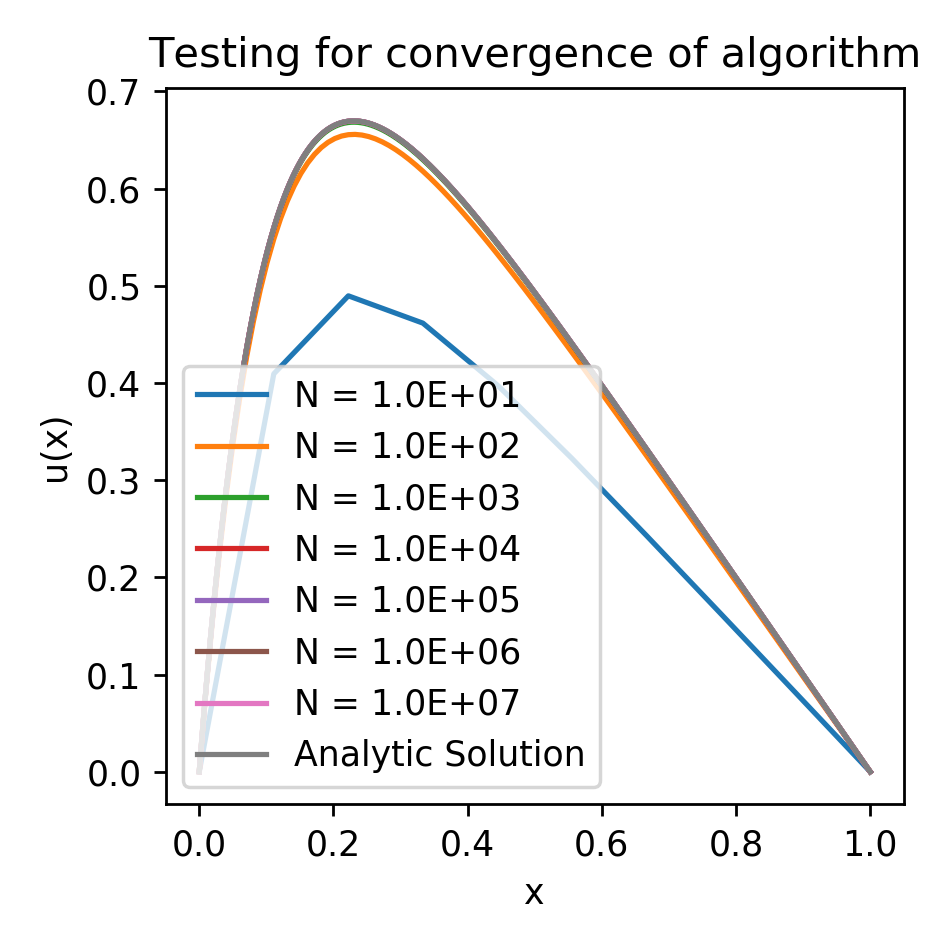
\includegraphics[scale=.7]{figs/ex1c_compare.png}
    \caption{A plot of the numeric solution for different N and the analytic solution.}
  \end{figure}

  \begin{figure}[hbtp]
    \center
    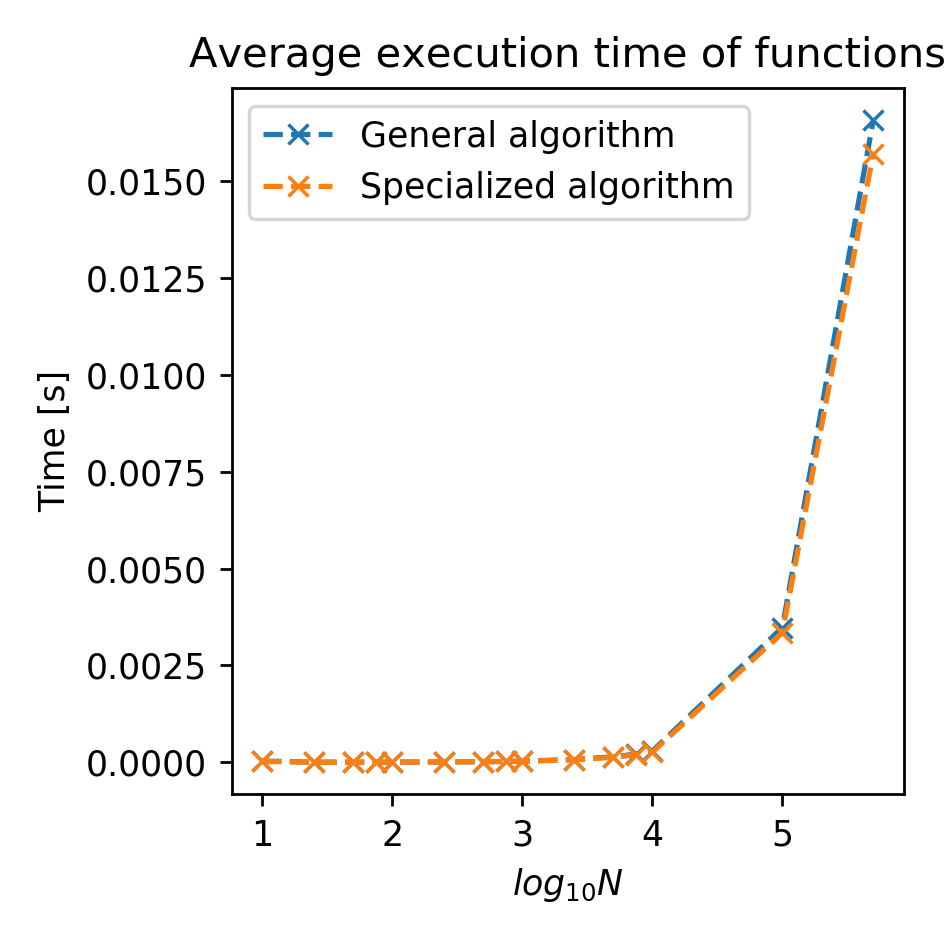
\includegraphics[scale=.7]{figs/ex1d_time.png}
    \caption{Comparing the average execution time of 100 function calls for the general and specialized algorithm.}
  \end{figure}

  \begin{figure}[hbtp]
    \center
    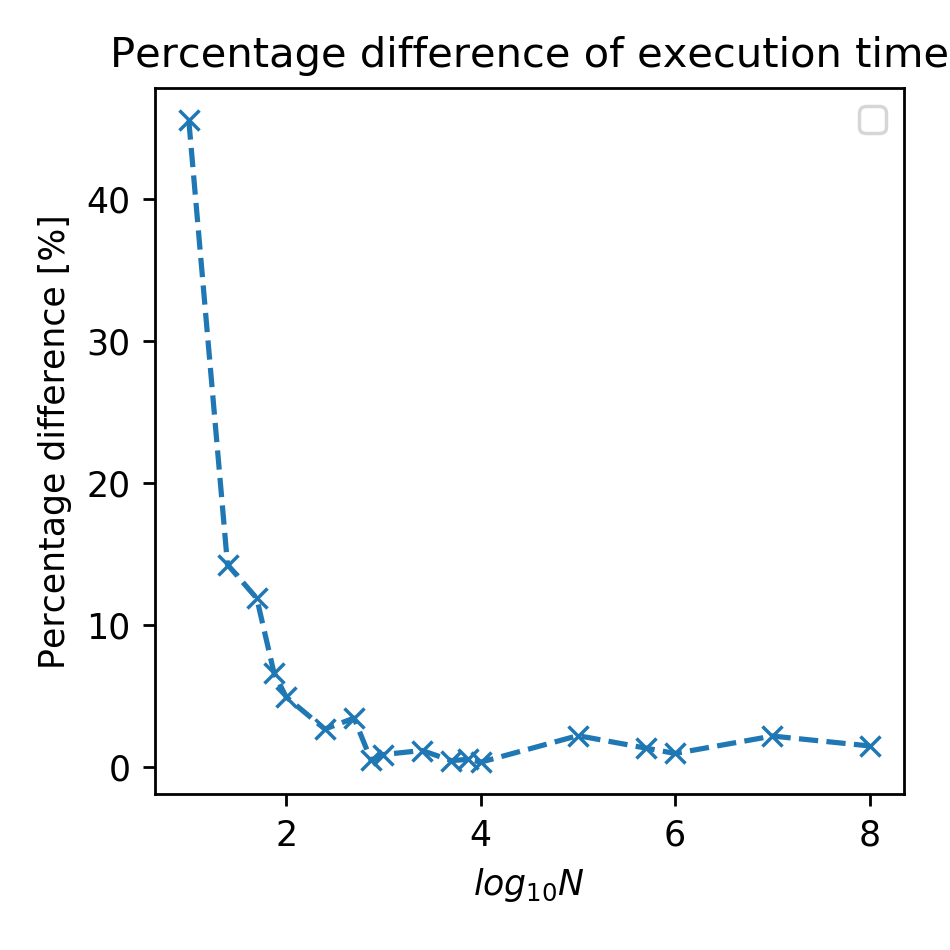
\includegraphics[scale=.7]{figs/ex1d_timediff.png}
    \caption{Percentage difference between the execution times of the general and specialized algorithms}
  \end{figure}




%\begin{figure}[hbtp]
%\includegraphics[scale=0.4]{test1.pdf}
%\caption{Exact and numerial solutions for $n=10$ mesh points.} 
%\label{fig:n10points}
%\end{figure}

\section{Conclusions}

\begin{thebibliography}{99}
\bibitem{lecture_notes} M.~Hjorth-Jensen, Computational Physics - Lecture Notes 2015, (2015).
\end{thebibliography}

\newpage

\appendix
  \section{Appendix}
  \begin{table}[h]
  \caption{PC Specifications}
  \begin{tabular}{|l|l|}
    \hline
    OS & Manjaro Linux \\ \hline
    CPU & Intel i7-4790K (8) @ 4.400GHz \\ \hline
    GPU & NVIDIA GeForce GTX 970  \\ \hline
    RAM & 15969MiB \\ \hline
  \end{tabular}
  \label{tab:specs}
  \end{table}


\end{document}